\documentclass[11pt,a4paper]{article}

\usepackage[T1]{fontenc}
\usepackage[utf8]{inputenc}
\usepackage{lmodern}
\usepackage{hyperref}
\usepackage{parskip}
\usepackage{enumitem}
\usepackage{geometry}
\geometry{margin=2.5cm}

\hypersetup{
  colorlinks=true,
  linkcolor=blue,
  urlcolor=blue
}

\title{Field Manual:\\Secure Passphrase Management with GnuPG and \texttt{pass}}
\author{%
  Practical Cross-Platform Operations Guide%
}
\date{\today}

\newcommand{\cmd}[1]{\texttt{#1}}
\newcommand{\file}[1]{\texttt{#1}}
\usepackage{graphicx}
\usepackage{titling}

% Cover page command
\newcommand{\makecover}{
  \begin{titlepage}
    \centering
    \vspace*{1cm}
    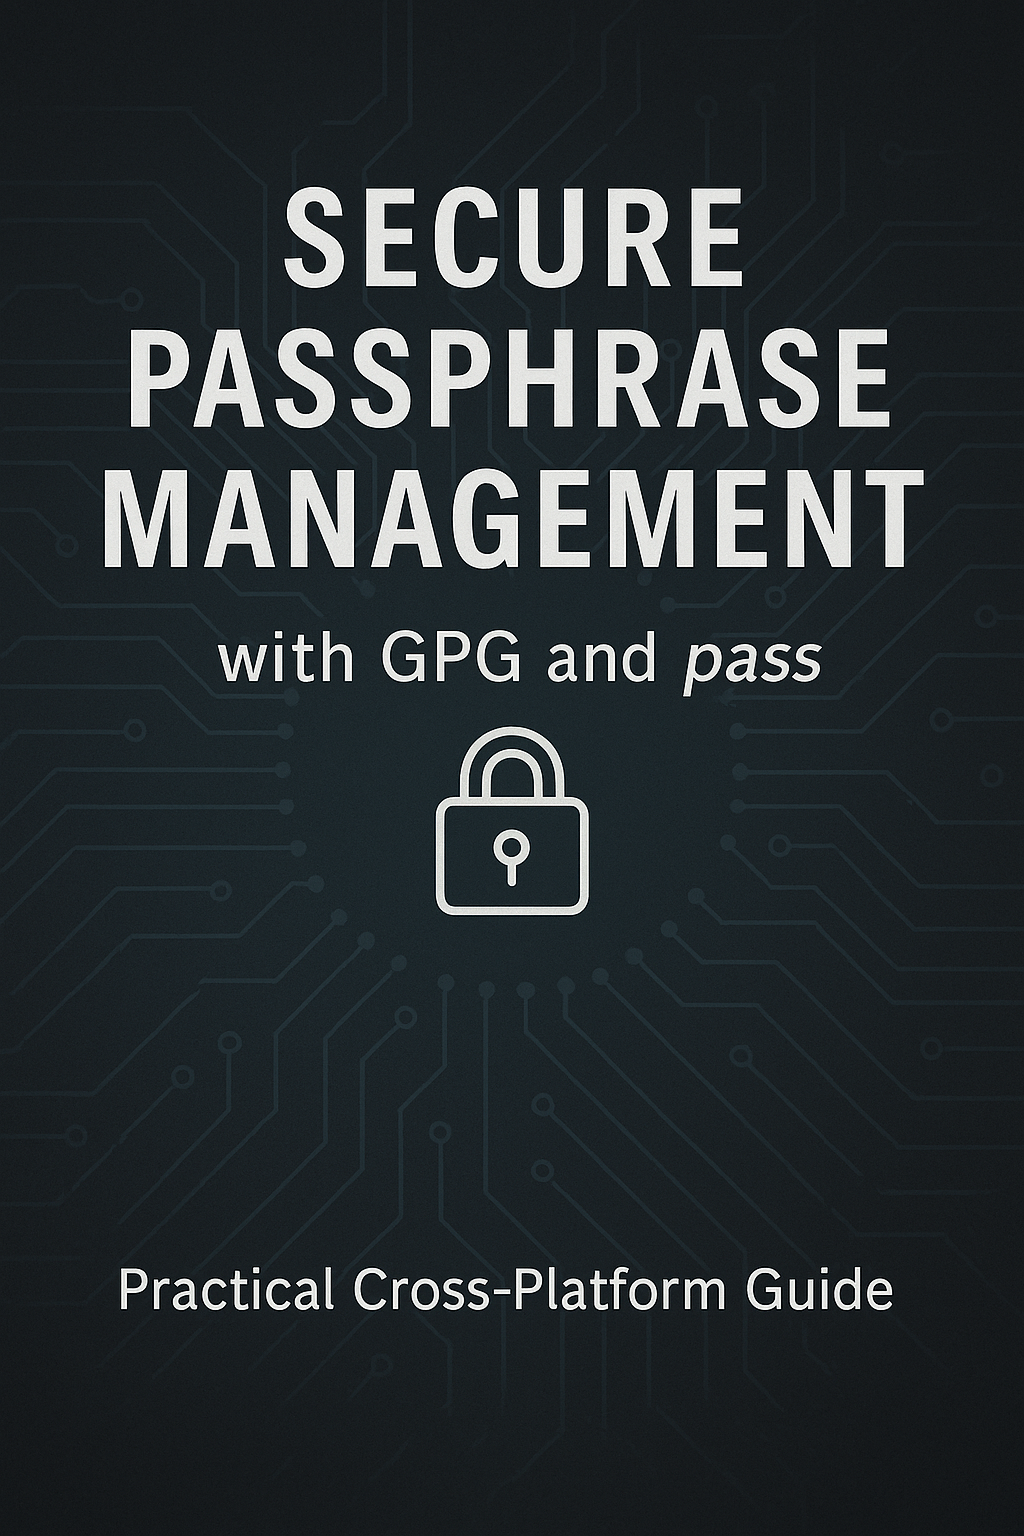
\includegraphics[width=0.85\textwidth]{cover_Secure_Passphrase_Management.png}
    \vfill
  \end{titlepage}
}


\begin{document}
\makecover

\maketitle

\tableofcontents
\newpage

\section{Introduction}

This field manual describes how to securely manage cryptographic passphrases, keys, and passwords using:

\begin{itemize}[noitemsep]
  \item \textbf{GnuPG (GPG)} -- for OpenPGP-compatible key management and encryption.
  \item \textbf{\texttt{pass} (password-store)} -- a simple, Unix-style password manager that stores each secret as an individual GPG-encrypted file.
\end{itemize}

The focus is on:

\begin{itemize}[noitemsep]
  \item Designing a robust passphrase strategy.
  \item Operating safely on Linux, macOS, and Windows.
  \item Implementing reliable backup and recovery procedures.
  \item Minimizing risk of irreversible data loss or compromise.
\end{itemize}

This manual assumes basic command-line familiarity but no prior crypto expertise.

\subsection{Threat Model and Goals}

We aim to defend against:

\begin{itemize}[noitemsep]
  \item Theft or loss of a laptop / phone.
  \item Compromise of a single cloud provider or sync service.
  \item Accidental deletion or disk failure on one device.
\end{itemize}

We explicitly \emph{do not} assume that:

\begin{itemize}[noitemsep]
  \item Your passphrases can resist a targeted nation-state forever.
  \item Your system is free of malware or keyloggers (this is a separate, but related, problem).
\end{itemize}

The operational goal is:

\begin{quote}
  \textbf{``If I lose one device or one backup, I lose nothing. If one provider is compromised, the attacker still cannot use my keys or passwords.''}
\end{quote}

\section{Installing GnuPG}

\subsection{Official GnuPG Resources}

\begin{itemize}[noitemsep]
  \item Main site: \url{https://www.gnupg.org/}
  \item Online manuals: \url{https://www.gnupg.org/documentation/manuals.html}
  \item GNU Privacy Handbook (GPH): \url{https://www.gnupg.org/gph/en/manual/book1.html}
\end{itemize}

Always prefer the packages from your OS vendor or the official installers linked from \url{https://www.gnupg.org/}.

\subsection{Linux}

On most Linux distributions:

\begin{verbatim}
# Debian/Ubuntu
sudo apt install gnupg

# Fedora
sudo dnf install gnupg2

# Arch Linux
sudo pacman -S gnupg
\end{verbatim}

After installation, verify:

\begin{verbatim}
gpg --version
\end{verbatim}

\subsection{macOS}

On macOS you have two main options:

\begin{enumerate}[noitemsep]
  \item \textbf{GPG Suite (GUI + CLI)}\\
        Official site: \url{https://gpgtools.org/}\\
        This includes a graphical key manager and integration with Mail.
  \item \textbf{Homebrew packages}\\
        \begin{verbatim}
        brew install gnupg pinentry-mac
        \end{verbatim}
        Then configure \cmd{gpg-agent} to use \cmd{pinentry-mac}.
\end{enumerate}

\subsection{Windows}

On Windows, the recommended distribution is:

\begin{itemize}[noitemsep]
  \item \textbf{Gpg4win} -- \url{https://www.gpg4win.org/}
\end{itemize}

Gpg4win includes GnuPG, a key manager (Kleopatra), and Outlook integration. During installation, keep defaults unless you know you need something specific.

\section{Creating and Managing GPG Keys}

\subsection{Key Strategy}

A sane baseline setup:

\begin{itemize}[noitemsep]
  \item One \textbf{primary key} for identity and certification.
  \item One or more \textbf{subkeys} for:
    \begin{itemize}[noitemsep]
      \item Encryption
      \item Signing
      \item Authentication (SSH, etc.)
    \end{itemize}
  \item A \textbf{strong passphrase} protecting the private primary key.
\end{itemize}

The primary key is rarely used and kept offline where possible; daily operations use subkeys.

\subsection{Generating a New Key}

Modern GnuPG:

\begin{verbatim}
gpg --full-generate-key
\end{verbatim}

Recommended choices:

\begin{itemize}[noitemsep]
  \item Key type: \texttt{(1) RSA and RSA} or \texttt{(9) ECC} (if you know what you are doing).
  \item Key size: at least 3072-bit RSA (4096 if you prefer).
  \item Expiry: 1--3 years, with the intention to extend as needed.
  \item User ID: real name or consistent handle + email.
  \item Passphrase: see Section~\ref{sec:passphrase-strategy}.
\end{itemize}

List keys:

\begin{verbatim}
gpg --list-keys
gpg --list-secret-keys
\end{verbatim}

\subsection{Revocation Certificate}

Immediately after creating a key, generate a revocation certificate and store it offline:

\begin{verbatim}
gpg --output revoke-cert.asc --gen-revoke yourkeyid
\end{verbatim}

Print or store \file{revoke-cert.asc} on offline media (e.g.\ encrypted USB, or paper via QR codes). Do \emph{not} keep it in the same place as your main key backups.

\subsection{Exporting Secret Keys for Backup}

Export your secret keys in an armored format:

\begin{verbatim}
gpg --export-secret-keys --armor yourkeyid > secret-keys.asc
gpg --export-secret-subkeys --armor yourkeyid > secret-subkeys.asc
\end{verbatim}

\textbf{Critical:} These files contain your private keys. Treat them like the physical keys to your house:

\begin{itemize}[noitemsep]
  \item Store them encrypted at rest (e.g.\ in an encrypted volume).
  \item Keep at least two physically separate copies (e.g.\ home safe + safety deposit box).
  \item Consider printing them as QR codes and storing in a sealed envelope.
\end{itemize}

\section{Installing and Using \texttt{pass}}

\subsection{Official \texttt{pass} Resources}

\begin{itemize}[noitemsep]
  \item Homepage: \url{https://www.passwordstore.org/}
  \item Project page: \url{https://git.zx2c4.com/password-store/about/}
\end{itemize}

\subsection{Installation}

Typical commands:

\begin{verbatim}
# Debian/Ubuntu
sudo apt install pass

# Fedora
sudo dnf install pass

# Arch Linux
sudo pacman -S pass

# macOS (Homebrew)
brew install pass
\end{verbatim}

On Windows, \texttt{pass} can be used via:

\begin{itemize}[noitemsep]
  \item WSL (Windows Subsystem for Linux).
  \item MinGW/MSYS2 or Cygwin builds.
\end{itemize}

In all cases, \texttt{pass} depends on GnuPG; ensure GPG is correctly installed first.

\subsection{Initializing the Password Store}

Choose a GPG key dedicated to your password store, or reuse your main key.

\begin{verbatim}
pass init "Your GPG Key ID or UID"
\end{verbatim}

This creates \file{\$HOME/.password-store} and configures it to encrypt entries to the specified key.

\subsection{Basic Operations}

\begin{description}[style=nextline]
  \item[Insert a new password:]
\begin{verbatim}
pass insert email/example.com
\end{verbatim}
    You will be prompted to type the password (twice).
  \item[Generate a random password:]
\begin{verbatim}
pass generate email/example.com 32
\end{verbatim}
    Generates a 32-character password and stores it.
  \item[Show a password:]
\begin{verbatim}
pass show email/example.com
\end{verbatim}
  \item[Copy to clipboard:]
\begin{verbatim}
pass -c email/example.com
\end{verbatim}
\end{description}

\subsection{Using Git for Sync and History}

\texttt{pass} integrates nicely with Git for versioning and synchronization.

\begin{verbatim}
cd ~/.password-store
git init
git remote add origin git@yourserver:pass-store.git
\end{verbatim}

From now on:

\begin{verbatim}
pass git status
pass git commit -am "Update password store"
pass git push
\end{verbatim}

This gives you:

\begin{itemize}[noitemsep]
  \item Version history of changes.
  \item Encrypted secrets replicated across devices.
\end{itemize}

Remember: the \textbf{content} is encrypted with GPG, but metadata (file names, Git commit messages, timestamps) may reveal which services you use.

\section{Passphrase Strategy}
\label{sec:passphrase-strategy}

\subsection{Principles}

\begin{enumerate}[noitemsep]
  \item A small number of \textbf{memorable, high-entropy passphrases} for master keys.
  \item Many \textbf{random, machine-generated passwords} for individual services.
  \item \textbf{Never} reuse master passphrases across different key sets or services.
\end{enumerate}

\subsection{Creating a Strong Master Passphrase}

Recommended approach:

\begin{itemize}[noitemsep]
  \item Use a Diceware-style passphrase: 6--8 random words from a large wordlist.
  \item Optionally add simple transformations you can remember, not complex rules.
  \item Example shape (do not use this exact one):\\
        \texttt{turtle amber north stairs cinema walnut}
\end{itemize}

Store this in your head, and optionally in a sealed offline record (e.g.\ written on paper, in a safe).

\subsection{Passwords Inside \texttt{pass}}

For each account:

\begin{itemize}[noitemsep]
  \item Use \cmd{pass generate} to create a long random password (24+ characters).
  \item Enable multi-factor authentication (TOTP, hardware key) where available.
  \item Store backup codes in \texttt{pass} under a descriptive path.
\end{itemize}

\subsection{GPG Agent and Pinentry}

GnuPG typically uses \cmd{gpg-agent} to cache your passphrase for a limited time.

Configure sensible cache lifetimes in \file{\$HOME/.gnupg/gpg-agent.conf}, for example:

\begin{verbatim}
default-cache-ttl 900      # 15 minutes
max-cache-ttl 3600         # 1 hour
\end{verbatim}

After editing, reload:

\begin{verbatim}
gpgconf --reload gpg-agent
\end{verbatim}

\textbf{Avoid} infinite caching; you want the agent to forget eventually.

\section{Backup and Recovery Procedures}

This section is the operational heart of the field manual.

\subsection{Backup Checklist (High Level)}

Maintain at least:

\begin{enumerate}[noitemsep]
  \item One primary device with your active GPG key and \texttt{pass} store.
  \item One secondary device that can be restored from backup and used in an emergency.
  \item Two independent offline backups of:
    \begin{itemize}[noitemsep]
      \item GPG secret keys and subkeys.
      \item Revocation certificates.
      \item \file{\$HOME/.password-store} Git repository.
    \end{itemize}
\end{enumerate}

\subsection{Backing Up GPG}

\subsubsection{Export Secret Keys and Subkeys}

As shown earlier:

\begin{verbatim}
gpg --export-secret-keys --armor yourkeyid > secret-keys.asc
gpg --export-secret-subkeys --armor yourkeyid > secret-subkeys.asc
\end{verbatim}

Encrypt these files again with a separate key or store them in an encrypted container (e.g.\ LUKS, VeraCrypt, FileVault, BitLocker).

\subsubsection{Backup Directory \texttt{\$HOME/.gnupg}}

Alternatively, back up the entire directory:

\begin{verbatim}
tar czf gnupg-backup.tar.gz ~/.gnupg
\end{verbatim}

\textbf{Warning:} This may include extra state (trustdb, random seed). Keep it well-protected.

\subsubsection{Physical and Geographic Separation}

For high assurance:

\begin{itemize}[noitemsep]
  \item Copy 1: Encrypted USB drive at home.
  \item Copy 2: Encrypted USB drive or printed key material in a separate secure location (office safe, safety deposit box).
\end{itemize}

\subsection{Backing Up the \texttt{pass} Store}

If you are using Git:

\begin{itemize}[noitemsep]
  \item Keep a remote bare repository (self-hosted or a trusted provider).
  \item Regularly \cmd{git push} after changes.
\end{itemize}

Additionally, periodically make a full archive:

\begin{verbatim}
tar czf password-store-backup.tar.gz ~/.password-store
\end{verbatim}

Store this archive alongside your GPG backups.

\subsection{Test Your Backups}

At least once per year:

\begin{enumerate}[noitemsep]
  \item Take a fresh system or VM.
  \item Import your GPG backup:
\begin{verbatim}
gpg --import secret-keys.asc
gpg --import secret-subkeys.asc
\end{verbatim}
  \item Clone or unpack your \texttt{pass} store:
\begin{verbatim}
git clone git@yourserver:pass-store.git ~/.password-store
\end{verbatim}
  \item Run \cmd{pass show some/entry} and verify you can decrypt.
\end{enumerate}

If any step fails, fix the process now. A backup you have never tested is a \emph{theory}, not a guarantee.

\section{Cross-Platform Usage}

\subsection{Sharing the Same Key and Store}

A common pattern:

\begin{enumerate}[noitemsep]
  \item Generate keys on your most secure, trusted machine.
  \item Create and back up keys and revocation certificates.
  \item Import secret keys onto secondary devices (laptops, desktops) as needed.
  \item Use Git to sync the \texttt{pass} store across devices.
\end{enumerate}

On each device:

\begin{verbatim}
# Import keys
gpg --import secret-keys.asc
gpg --import secret-subkeys.asc

# Clone password store
git clone git@yourserver:pass-store.git ~/.password-store

# Check pass works
pass ls
\end{verbatim}

\subsection{Mobile Access}

Mobile options change over time, but the typical pattern is:

\begin{itemize}[noitemsep]
  \item A pass-compatible app that:
    \begin{itemize}[noitemsep]
      \item Syncs via a Git repository or file sync (e.g.\ SSH, WebDAV, cloud drive).
      \item Uses your OpenPGP key (imported or via hardware token).
    \end{itemize}
\end{itemize}

Treat mobile devices as higher risk:

\begin{itemize}[noitemsep]
  \item Require device-level full-disk encryption.
  \item Use a longer device unlock PIN or passphrase.
  \item Consider using subkeys only (not the primary key) on mobile.
\end{itemize}

\section{Operational Practices}

\subsection{Rotation and Hygiene}

\begin{itemize}[noitemsep]
  \item Periodically extend key expiry and review keys.
  \item Rotate passwords for sensitive accounts (email, banking, domain registrars).
  \item Remove dormant accounts where possible.
\end{itemize}

\subsection{When You Suspect Compromise}

If you believe your master GPG key or passphrase may be compromised:

\begin{enumerate}[noitemsep]
  \item Stop using the compromised key immediately.
  \item Use the revocation certificate to revoke the key.
  \item Generate a new key pair and new password-store key if needed.
  \item Migrate critical passwords to secrets encrypted under the new key.
  \item Review important accounts (email, banks, cloud providers) and rotate credentials.
\end{enumerate}

\section{Appendix A: Minimal Command Reference}

\subsection{GnuPG}

\begin{verbatim}
# Generate a new key
gpg --full-generate-key

# List public keys
gpg --list-keys

# List secret keys
gpg --list-secret-keys

# Export public key
gpg --export --armor yourkeyid > pubkey.asc

# Export secret keys
gpg --export-secret-keys --armor yourkeyid > secret-keys.asc

# Import keys
gpg --import somekey.asc

# Generate revocation cert
gpg --output revoke-cert.asc --gen-revoke yourkeyid
\end{verbatim}

\subsection{\texttt{pass}}

\begin{verbatim}
# Initialize password store
pass init "Your GPG Key ID or UID"

# Insert password
pass insert category/service

# Generate password
pass generate category/service 32

# Show password
pass show category/service

# Copy password to clipboard
pass -c category/service

# List stored entries
pass ls

# Use git integration
pass git status
pass git commit -am "Update secrets"
pass git push
\end{verbatim}

\section{Appendix B: Official Resources and Further Reading}

\subsection{GnuPG}

\begin{itemize}[noitemsep]
  \item Official website: \url{https://www.gnupg.org/}
  \item Manuals (HTML/PDF): \url{https://www.gnupg.org/documentation/manuals.html}
  \item GNU Privacy Handbook: \url{https://www.gnupg.org/gph/en/manual/book1.html}
  \item Windows distribution (Gpg4win): \url{https://www.gpg4win.org/}
  \item macOS GPG Suite: \url{https://gpgtools.org/}
\end{itemize}

\subsection{\texttt{pass} / Password Store}

\begin{itemize}[noitemsep]
  \item Official website: \url{https://www.passwordstore.org/}
  \item Project page and documentation: \url{https://git.zx2c4.com/password-store/about/}
  \item Manual page (Linux manpages mirror): \url{https://man.archlinux.org/man/pass.1.en}
\end{itemize}

\subsection{General Password-Management Guidance}

For broader operational security and password-management guidance, consult your operating system's security documentation and reputable infosec resources. Always verify that advice is current and comes from trusted sources.

\end{document}
